\documentclass[../Interim_Report_Master]{subfiles}
\begin{document}
\hypertarget{back_mat}{\section{Background Material}\label{back_mat}}
\subsection{GPU Computing}
\begin{wrapfigure}[14]{r}{0.5\textwidth}
	\vspace{-1\intextsep}
	\begin{tikzpicture}[node distance=6cm, >=latex, thick, scale=0.5]
	\tikzstyle{CPU} = [rectangle, draw=black, minimum width=3cm, minimum height=2cm, text centered]
	\tikzstyle{MEM} = [rectangle, draw=black, minimum width=3cm, minimum height=1cm, text centered]
	\node (CPU_L) [CPU] {CPU Threads};
	\node (CPU_R) [CPU, right=2cm of CPU_L] {CPU Threads};
	\draw[<->] (CPU_L.east) -- (CPU_R.west) node[midway,above]{MPI};
	\node (MEM_L) [MEM, above=2cm of CPU_L] {Memory};
	\node (MEM_R) [MEM, above=2cm of CPU_R] {Memory};
	\draw[<-](-0.5,2)--(-0.5,6);
	\draw[->](0.5,2)--(0.5,6);
	\draw[<-](9.5,2)--(9.5,6);
	\draw[->](10.5,2)--(10.5,6);
	\foreach \x in {-2,...,2}{
		\draw (\x,-2)--(\x, -0.5);
		\draw(\x,0.5)--(\x, 2);
	}
	\foreach \x in {8,...,12}{
		\draw (\x,-2)--(\x, -0.5);
		\draw(\x,0.5)--(\x, 2);
	}
	\end{tikzpicture}
	\caption{MPI block diagram.}
	\label{MPI}
\end{wrapfigure}

The question, why use GPUs? Naturally arises from the title of this project. CPUs in large computing clusters like the University of Southampton's Iridis Compute Cluster could be used. This would simplify the project as extra code called a kernel has to be written for the simulation to run on a GPU. The problem arises in the way CPUs share data in computing clusters.To write code for CPU parallel computing MPI has to be used. A block diagram of this is shown in Figure \ref{MPI}.

This process of sharing data between compute nodes is what really limits CPU parallel computing. The overhead this adds would cause simulations not to scale linearly compared with using a GPU for a highly parallel task. As by comparison the GPU threads are able to access the same shared memory as shown in Figure \ref{GPU}. With regards to writing GPU kernels there are two languages to choose from. The Open Computing Language, OpenCL and the Compute Unified Device Architecture, CUDA. CUDA is a language developed by Nvidia that only runs on Nvidia GPUs, whereas OpenCL is open source and can run any GPU and indeed a wider range of compute devices. The existing code uses OpenCL kernels, to enable greater hardware compatibility, so OpenCL is the language that will be used for this project. 

\begin{figure}
\centering
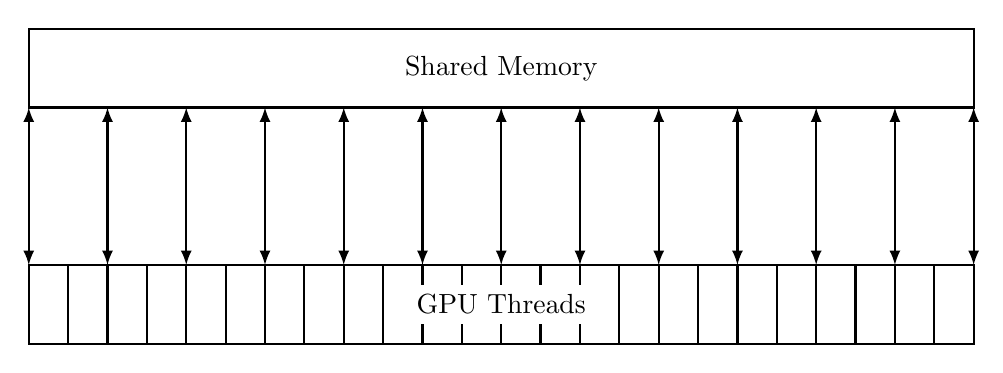
\begin{tikzpicture}[node distance=3cm, >=latex, thick, scale=0.5]
	\tikzstyle{rect} = [rectangle, draw=black, minimum width=12cm, minimum height=1cm, text centered]
	\node (GPU) [rect] {GPU Threads};
	\node (GPU_MEM) [rect, above of=GPU] {Shared Memory};
	\foreach \x in {-12,-10,...,12}
	\draw[<->] (\x,1)--(\x, 5);
	\foreach \x in {-12,...,-3}
	\draw (\x,-1)--(\x, 1);
	\foreach \x in {3,...,12}
	\draw (\x,-1)--(\x, 1);
	\foreach \x in {-4,...,4}{
		\draw (\x,-1)--(\x, -0.5);
		\draw (\x,0.5)--(\x, 1);
	}
\end{tikzpicture}
\caption{GPU memory block diagram.}
\label{GPU}
\end{figure}

\newpage

\subsection{Physics of Droplet Evaporation}
\subsubsection{Heat Transfer Processes}
Fundamental to modelling droplets is an understanding of multiphase fluids. Droplet laden flows, (the subject of this report) are an example of two phase flows.

With regards to the physics of droplet evaporation there are two fundamental driving processes. These are diffusion and convection.

Diffusion is a process where there is a net movement of particles from a region of high concentration to a region of low concentration. This is driven by the concentration gradient so is affected by properties of the particles and the distance over which diffusion occurs. The carrier species of the particles will also affect the flux. Fick's Law quantifies this as:
\begin{equation}
J(x,y,z) = -d\left(\frac{\partial C}{\partial x},\frac{\partial C}{\partial y},\frac{\partial C}{\partial z}\right)
\end{equation}
\cite{Nazaroff2001}.

More useful is thermal diffusion, with the rate defined by Fourier's Law. For example, in one dimension as:
\begin{equation}
\dot{q}_x=-k\frac{dT}{dx}
\end{equation}

With $x$ in the direction of heat transfer, $\dot{q}_x$ the heat transfer rate per unit area, $k$ the thermal conductivity and $dT/dx$ the temperature gradient in the $x$-direction. \cite{Deiterding2019}

Convection transfers heat energy in the direction of motion of the fluid. Convection can be forced (some fluid flow forcing convective transfer), or natural (the flow is created by the forces resulting from the heat transfer). Convective heat transfer for a fluid is given by:
\begin{equation}
\dot{q} = h\Delta T
\end{equation}

where $\Delta T$ is the difference between the temperature at the surface of the fluid and the temperature at infinity: $T_s-T_{\infty}$. The convective heat transfer coefficient $h$ contains variables that allow for a simple form for the convective heat transfer equation.\cite{Shrimpton2015}

In general an exact solution for $h$ is only available for specific cases such as laminar flow. More common is to form an empirical relation using non-dimensional numbers that capture the physics of the problem. \cite{Deiterding20192}

\subsubsection{Vapour Pressure}
The driving force for changes to the properties in the vapour phase is the vapour pressure. Assuming the droplet is formed of a pure liquid species the vapour pressure is only a function of temperature. For evaporation to occur the partial pressure of the liquid must be less than the vapour pressure \cite{Nazaroff2001}. 

The vapour pressure can be found by considering that for two phases to be in equilibrium their respective chemical potentials, $\mu_{pot}$ must be equal. This implies here that $\mu_{liquid}=\mu_{gas}$ and any changes must be equal $\to d\mu_{liquid}=d\mu_{gas}$. If there is a change of pressure acting on the liquid phase, i.e. $dV_{m, liquid}dP=d\mu_{liquid}$. (With $dV_{m, liquid}$ the molar volume of the liquid phase). Therefore, $dV_{m, gas}dP_{vapour}=d\mu_{gas}$, with $dP_{vapour}$ the change in vapour pressure. Equating the changes in the liquid and gas phase, it is possible using integration and assuming the gas is perfect and the molar volume of gas is much greater than the molar volume of the liquid to derive the Clausius-Clapeyron equation. \cite{atkins_paula_2010}

\begin{equation}
\chi_{s,eq} = \frac{P_{atm}}{P_G}\exp \left[\frac{L_V}{\bar{R}/W_V}\left(\frac{1}{T_B}-\frac{1}{T_d}\right)\right] 
\end{equation}

So the equilibrium mole fraction of the vapour can be found.

\subsubsection{Mass Transfer}

%Deriving mass and heat transfer requires applying their respective conservation laws. For conservation of mass, the rate of mass lost by the droplet must be equal to the mass that is evaporated:
%
%
%
%The droplet will also be at some temperature $T_d$. To model what takes place at the surface of the droplet consider Figure x:
%
%
%
%The heat energy applied by the the gas surrounding the droplet is $Q_S$. with the 


\subsubsection{Droplet Physical Model}
The droplet consists of a a liquid phase surrounded by a vapour phase, with the droplet surrounded by a gas phase which is the carrier gas species. A diagram of the physical model of the droplet is shown in Figure x.
\begin{figure}[h]
	\centering
	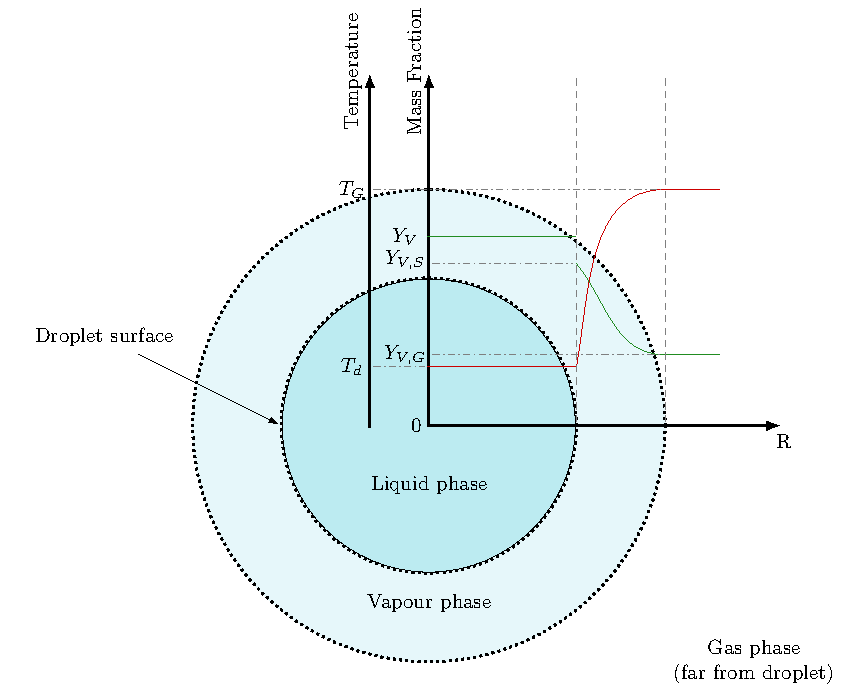
\includegraphics[width=0.8\textwidth]{./Diagrams/Droplet_Diagram/Droplet_Diagram.pdf}
	\caption{Diagram of how the droplet's and carrier gas phases with their associated properties vary with droplet radius.}
	\label{drop_diag}
\end{figure}

The droplet temperature is assumed to be uniform within the droplet, although various with time. This. In reality there is a thermal gradient across the droplet. The internal temperature profile can be modelled as part of M8 in \cite{Miller1998}. The temperature rises across the vapour phase to the gas temperature. 

Similarly within the droplet the mass fraction of droplet vapour within the droplet is uniform and is equal to 1. The mass fraction drops instantaneously at the surface, as the surface of the droplet is a mixture of droplet vapour and gas phase. The mass fraction of vapour decreases across the vapour phase until an equilibrium mixture with the gas phase phase is reached. 

 \cite{pinheiro_vedovoto_2018}.


%For developing a simulation code to model the physics of droplets it is impractical to model the droplets as three dimensional fluid objects with the associated boundary layers, etc... Especially given the code must be robust and efficient enough to allow for a large population of particles to be simulated in a reasonable time. Therefore, each droplet is considered as a point mass and the physics of what process are taking place on the droplet are modelled. 
%
%The first assumption made in deriving a model is the droplet is spherical, with mass $m_d$ and diameter $D$. With mass and diameter related by:
%\begin{subequations}
%	\begin{eqnarray}
%	m_d =& \rho_d V_d \\
%	=& \rho_d \left(\frac{4}{3}\right) \pi \left(\frac{D}{2}\right)^3 \\
%	=& \frac{\rho_d \pi D^3}{6}
%	\end{eqnarray}
%\end{subequations}
%Where $\rho_d$ is the droplet density, assumed to be constant.

\end{document}